%%Énoncé
L'ordre d'insertion des clés dans un AVL a t-il une influence sur la forme finale de l'arbre ?
Jamais, parfois, toujours ? Justifiez vos réponses.
Dessinez un arbre AVL de hauteur 5 ayant un nombre minimal de nœuds. Que peut-on
dire de la relation entre hauteur h et nombre de nœuds n dans un arbre AVL ? \textit{(Jonathan)} \\
%%Réponse
\\ Oui, l'ordre d'insertion des clés dans un AVL à parfois de l'influence sur la forme finale de l'arbre.

Prenons le cas simple d'un arbre avec seulement deux clés 1 et 2.
Suivant l'ordre dans lequel on insère les clés, la forme final de l'arbre sera différent.
\\

\begin{tabular}{ll}
    Soit 1 puis 2 & Soit 2 puis 1 \\
   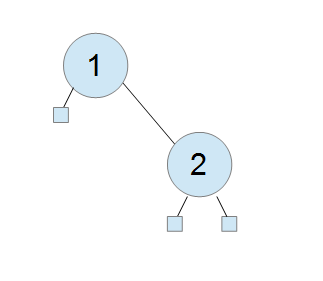
\includegraphics[scale=0.55]{1-2.png} & 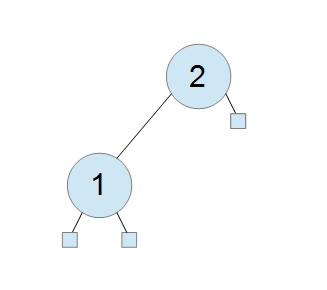
\includegraphics[scale=0.55]{2-1.png} \\


\end{tabular}

Ou bien encore pour un arbre avec 5 clés \\

\begin{tabular}{ll}
  Ordre : 3-2-1-4-5 & Ordre : 4-1-5-3-2 \\ 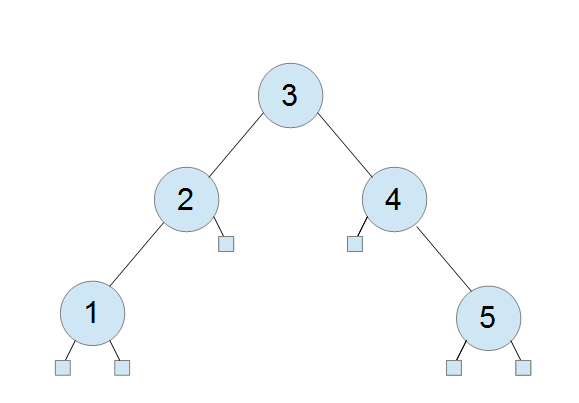
\includegraphics[scale=0.30]{3-2-1-4-5.png} & 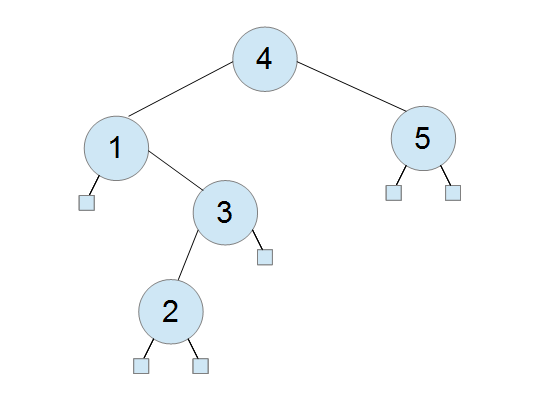
\includegraphics[scale=0.30]{4-1-5-3-2(nonequi).png} \\
  
\end{tabular}

Cependant ces deux arbres ne sont pas des arbre AVL, il faut prendre en compte la propriété d'équilibre. On obtient donc les arbres ci dessous.\\

\begin{tabular}{ll}
  Ordre : 3-2-1-4-5 AVL & Ordre : 4-1-5-3-2 AVL \\ 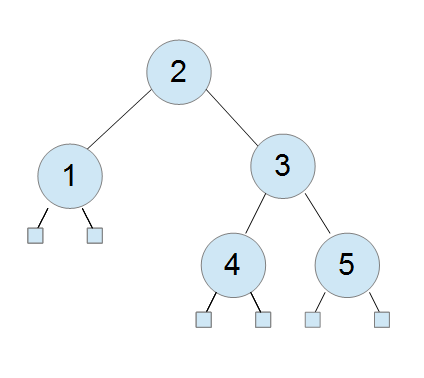
\includegraphics[scale=0.40]{3-2-1-4-5(equi).png} & 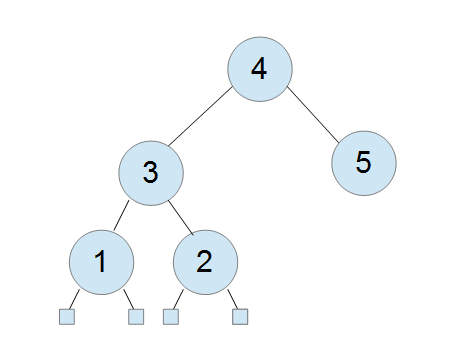
\includegraphics[scale=0.40]{4-1-5-3-2(equi).png} \\
  
\end{tabular}

On remarque bien que l'ordre des clés a vraiment de l'importance pour la forme finale de l'arbre. Cependant, parfois ce n'est pas le cas. Prenons un exemple avec un AVL qui possède 3 clés 1, 2 et 3.
dans l'ordre : 1-2-3 ou dans l'ordre : 3-2-1 on obtient le même arbre grâce à la propriété d'équilibre. Celui-ci est représenté ci dessous.
 

\begin{figure}[!h]
	\centering
	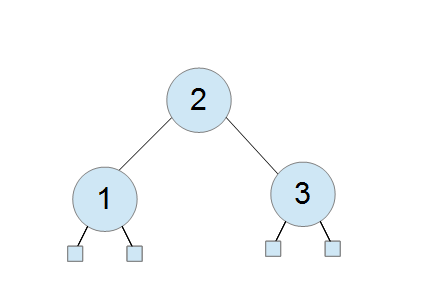
\includegraphics[scale=0.50]{123.png}
	\caption{Arbre AVL}
	\label{fig:equi}
\end{figure}

C'est deux cas différents simple mais efficace, nous permis de prouver que dans la plupart des cas l'autre des clés à de l'influence sur la forme finale de l'arbre.

Voici un arbre AVL de hauteur 5 ayant un nombre minimal de nœuds
De manière générale, on peut borner la hauteur d'un arbre binaire équilibré en fonction du nombre $n$ d'entrées par la relation suivante :
$$log( n ) \leq h \leq 2 \cdot log( n ) + 2$$
que l'on peut aussi exprimer comme suivant : $2^{(h/2 - 1)} \leq n \leq 2^h - 1$.

\begin{figure}[!h]
	\centering
	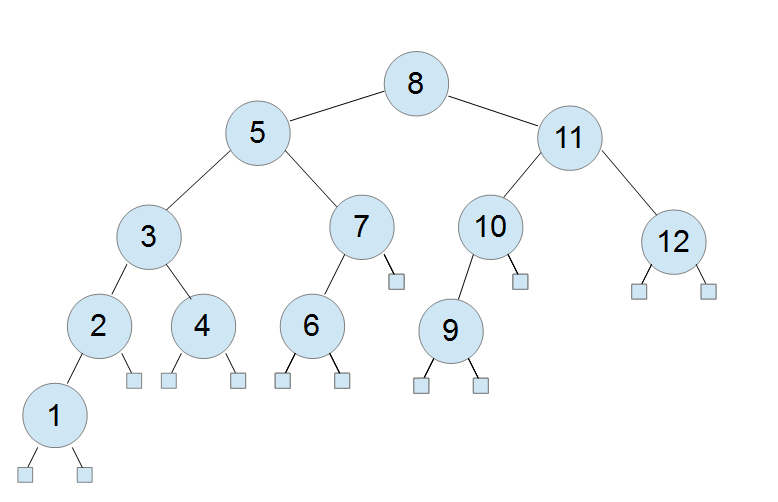
\includegraphics[scale=0.50]{hauteur5.png}
	\caption{Arbre AVL de hauteur 5 avec un nombre minimal de nœuds}
	\label{fig:equi}
\end{figure}
